% !TEX TS–program = pdflatexmk
\documentclass[12pt,a4paper,oneside,openany]{article}
\usepackage[squaren]{SIunits}
%% LaTeX Preamble - Common packages
\usepackage[english]{babel}
\usepackage{setspace}

\usepackage{fancyhdr}
\pagestyle{fancy}
%\cfoot{\thepage{} – CONFIDENTIAL}


\usepackage[utf8]{inputenc} % Any characters can be typed directly from the keyboard, eg éçñ
\usepackage{textcomp} % provide lots of new symbols
\usepackage{graphicx}  % Add graphics capabilities
\usepackage{flafter}  % Don't place floats before their definition
%\usepackage{topcapt}   % Define \topcaption for placing captions above tables (not in gwTeX)
%\usepackage{natbib} % use author/date bibliographic citations
%\usepackage{babelbib}
\usepackage[backend=biber]{biblatex}
\addbibresource{n17-servo-design.bib}

\usepackage{subfig}
\usepackage{caption}
\usepackage{enumitem}

\usepackage{amsmath,amssymb}  % Better maths support & more symbols
\usepackage{bm}  % Define \bm{} to use bold math fonts
\usepackage{esint}
\usepackage{algorithm}
\usepackage{mathenv}
%\usepackage[noend]{algorithmic}
\usepackage{algorithmicx}
\usepackage{algpseudocode}
\usepackage[usenames,dvipsnames]{color} 

\usepackage[pdftex,bookmarks,colorlinks,breaklinks]{hyperref}  % PDF hyperlinks, with coloured links
%\definecolor{dullmagenta}{rgb}{0.4,0,0.4}   % #660066
%\definecolor{darkblue}{rgb}{0,0,0.4}
\hypersetup{linkcolor=red,citecolor=blue,filecolor=blue,urlcolor=blue} % coloured links
%\hypersetup{linkcolor=black,citecolor=black,filecolor=black,urlcolor=black} % black links, for print output

\usepackage{memhfixc}  % remove conflict between the memoir class & hyperref
% \usepackage[activate]{pdfcprot}  % Turn on margin kerning (not in gwTeX)
%\usepackage{pdfsync}  % enable tex source and pdf output syncronicity

\usepackage{longtable}
\usepackage{booktabs}
\usepackage{listings}
\usepackage{nomencl}
\usepackage{todonotes}

\usepackage[noabbrev]{cleveref}

\usepackage{tablefootnote}
%\makesavenoteenv{tabular}

\usepackage{tikz}
\usetikzlibrary{calc,arrows,through,backgrounds,fit,shapes.geometric,shapes.misc,plotmarks,positioning,trees}
\usepackage{circuitikz}

%\usepackage{sagetex}

%\usepackage{anysize}
%\marginsize{2cm}{2cm}{2cm}{2cm}

\onehalfspacing

\makenomenclature
\def\nomlabel#1{\textbf{#1}\hfil}

%\newcommand{\Parameters}{\subsection*{Parameters}}
%\newcommand{\ReturnValue}{\subsection*{Return Value}}
%\newcommand{\Description}{\subsection*{Description}}
%\newcommand{\ClassName}[1]{{\tt #1}}
%\newcommand{\ReturnType}[1]{{\tt (#1)}}
%\newcommand{\Function}[1]{{\tt #1()}}
%\newcommand{\Self}{{\tt self}}

\DeclareMathOperator{\ud}{d}
\DeclareMathOperator{\udt}{\frac{d}{dt}}
%\DeclareMathOperator{\udtt}{\frac{\ud^2}{\ud t^2}}
\DeclareMathOperator{\rank}{rank}
\DeclareMathOperator{\fclamp}{clamp}
\DeclareMathOperator{\fsign}{sign}
%\newcommand{\ud}{\ensuremath{\binop{\mathrm{d}}}}
\newcommand{\vx}{\ensuremath{\mathbf{x}}}
\newcommand{\vy}{\ensuremath{\mathbf{y}}}
\newcommand{\vz}{\ensuremath{\mathbf{z}}}
\newcommand{\vu}{\ensuremath{\mathbf{u}}}
\newcommand{\vv}{\ensuremath{\mathbf{v}}}
\newcommand{\vw}{\ensuremath{\mathbf{w}}}
\newcommand{\va}{\ensuremath{\mathbf{a}}}
\newcommand{\vf}{\ensuremath{\mathbf{f}}}
\newcommand{\vt}{\ensuremath{\mathbf{t}}}
\newcommand{\vk}{\ensuremath{\mathbf{k}}}
\newcommand{\mM}{\ensuremath{\mathbf{M}}}
\newcommand{\mW}{\ensuremath{\mathbf{W}}}
\newcommand{\mJ}{\ensuremath{\mathbf{J}}}
\newcommand{\mA}{\ensuremath{\mathbf{A}}}
\newcommand{\mB}{\ensuremath{\mathbf{B}}}
\newcommand{\mH}{\ensuremath{\mathbf{H}}}
\newcommand{\vq}{\ensuremath{\mathbf{q}}}
\newcommand{\mC}{\ensuremath{\mathbf{C}}}
\newcommand{\mK}{\ensuremath{\mathbf{K}}}
\newcommand{\mP}{\ensuremath{\mathbf{P}}}
\newcommand{\mQ}{\ensuremath{\mathbf{Q}}}
\newcommand{\mR}{\ensuremath{\mathbf{R}}}
\newcommand{\vlambda}{\ensuremath{\boldsymbol{\lambda}}}
\newcommand{\vd}{\ensuremath{\mathbf{d}}}
\newcommand{\mI}{\ensuremath{\mathbf{I}}}
\newcommand{\vc}{\ensuremath{\mathbf{c}}}
\newcommand{\vr}{\ensuremath{\mathbf{r}}}
\newcommand{\vF}{\ensuremath{\mathbf{F}}}
\newcommand{\vtau}{\ensuremath{\boldsymbol{\tau}}}
\newcommand{\valpha}{\ensuremath{\boldsymbol{\alpha}}}

\newtheorem{mydef}{Definition}


\lstset{numbers=left,basicstyle=\footnotesize\ttfamily,numberstyle=\tiny,tabsize=4,breaklines=true}
\lstset{language=[Objective]C}
\lstset{commentstyle=\color{BrickRed}\itshape,
	keywordstyle=\color{RoyalBlue}\bfseries,
	identifierstyle=\color{Blue},
	stringstyle=\color{Gray}}

\long\def\symbolfootnote[#1]#2{\begingroup%
\def\thefootnote{\fnsymbol{footnote}}\footnote[#1]{#2}\endgroup}


\begin{document}


\title{Servo Controller Design Notes}
\author{Dömötör Gulyás\\v0.1}

\maketitle

%\abstract
%
%foopsum.
%
%

\tableofcontents

%\listoffigures

%\section{Introduction}

%\begin{figure}[htbp]
%\begin{center}
%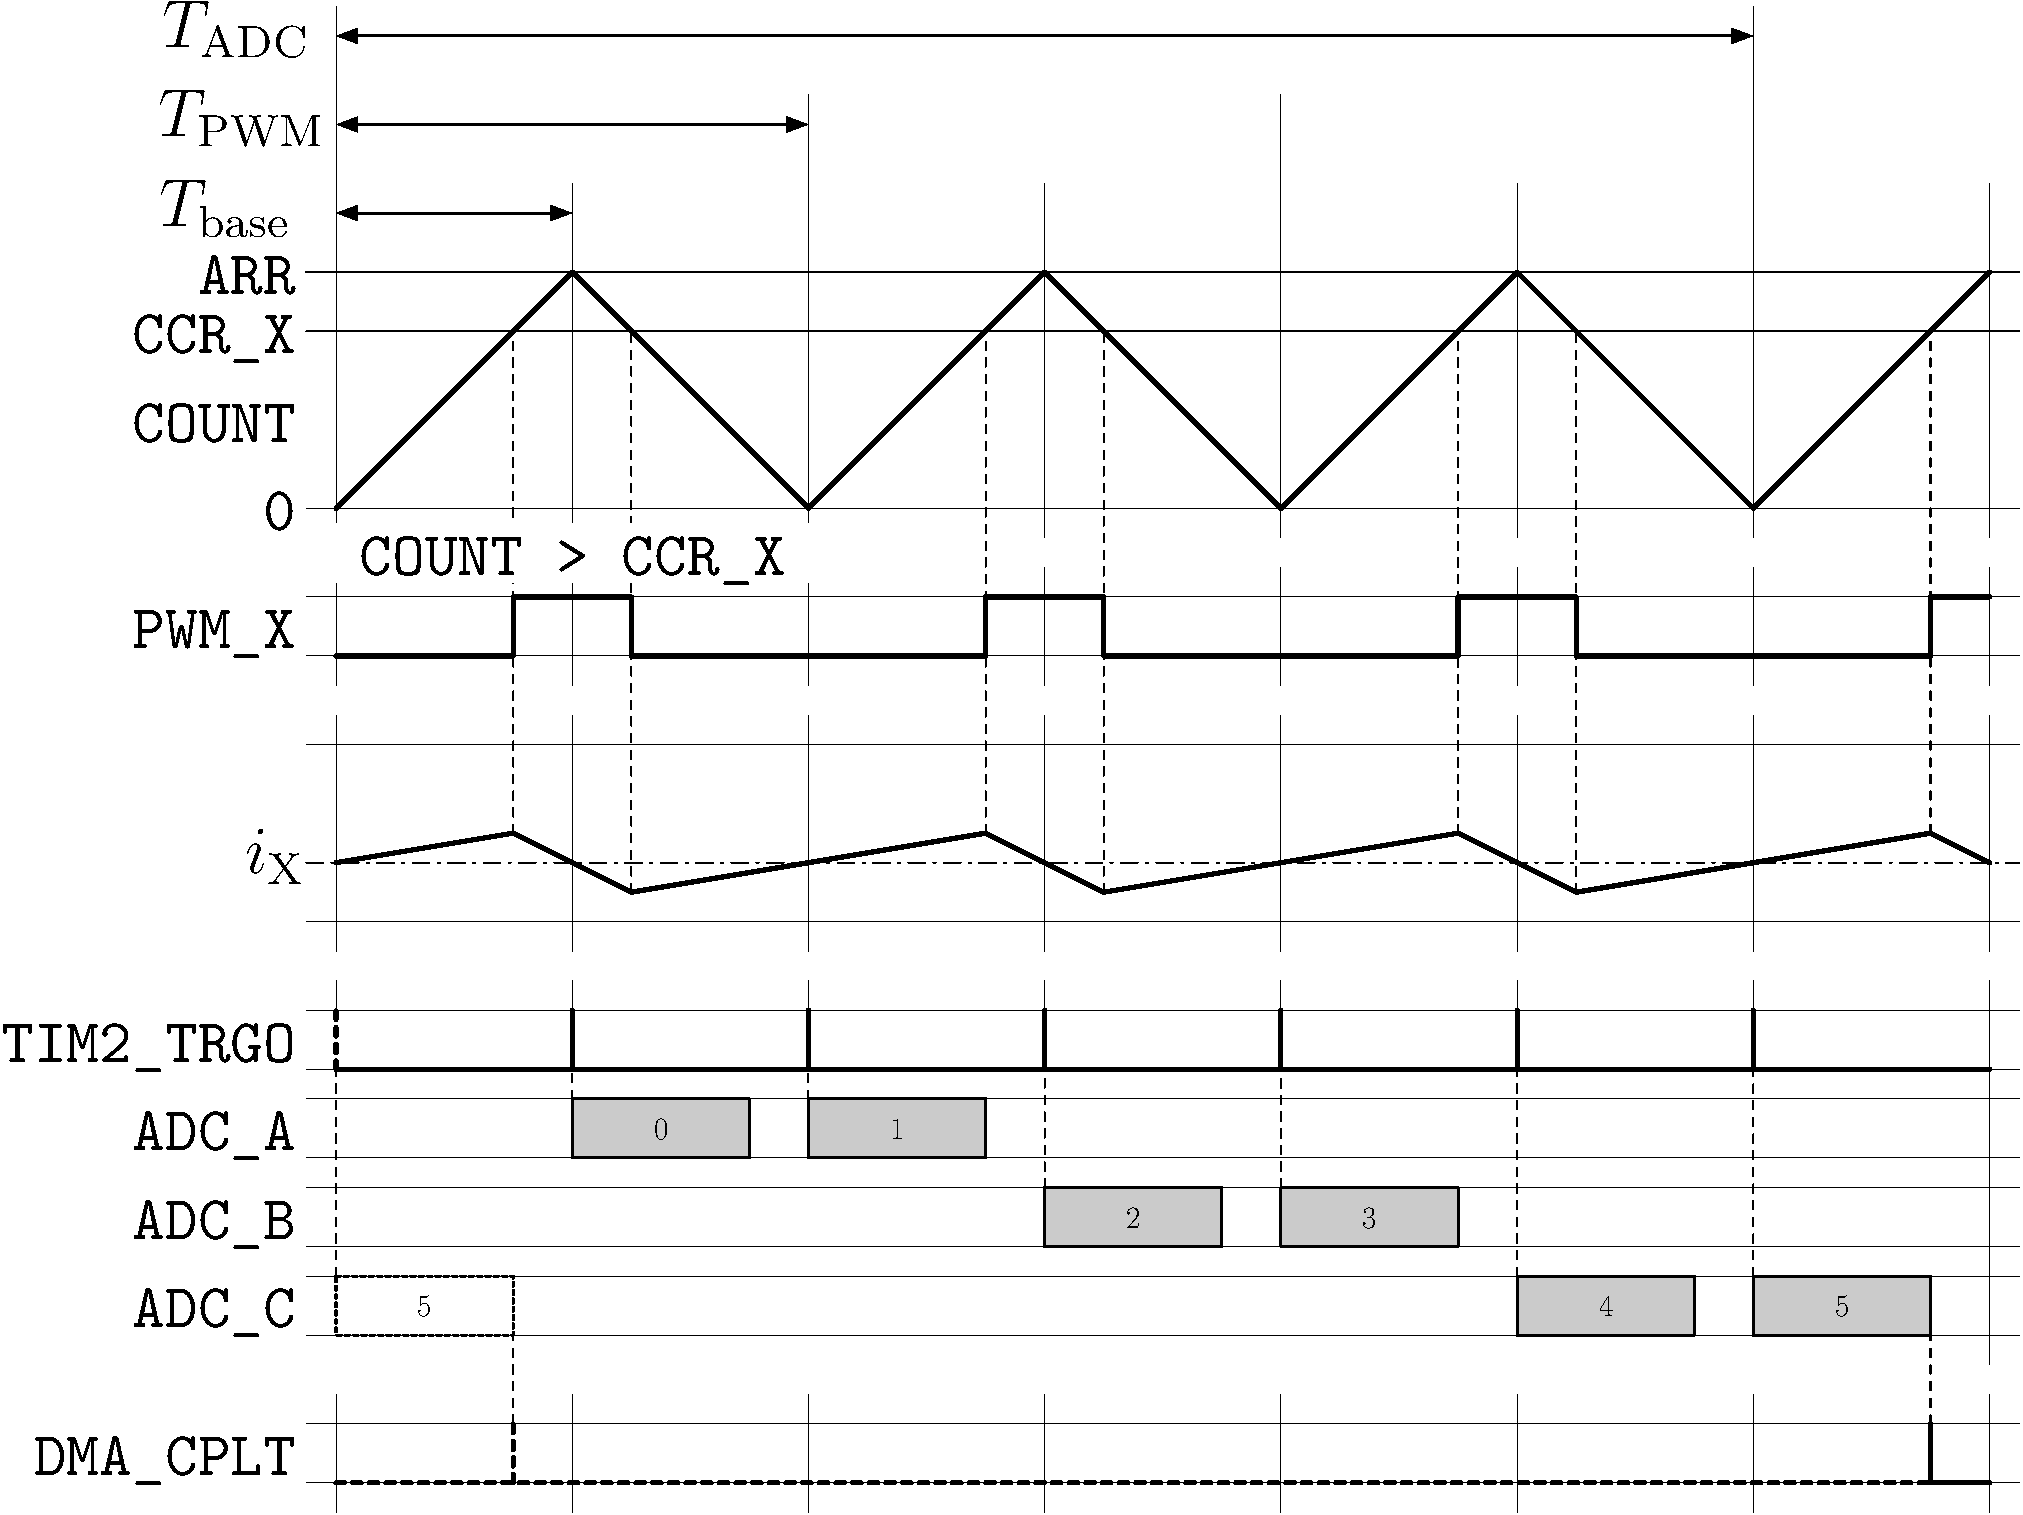
\includegraphics[scale=0.8]{n17-servo-pwm-adc.pdf}
%\caption[Fig]{foo}
%\label{fig:pwm-adc}
%\end{center}
%\end{figure}

\section{Hardware}

The hardware is laid out to be as flexible as possible, driving both 3-phase BLDC and servo motors, as well as 2-phase steppers.

3 half bridges with discrete transistors allow high currents. The DRV8323 stepper driver works at up to 60V. The hardware is laid out for 12V-48V nominal voltage, but allowing 60V peak.

Using a 2-phase motor in this configuration limits the top speed due to lower effective voltage than one could get using 2 full bridges.

The main MCU is an STM32G431.

\subsection{SPI}

Unfortunately the STM32G4 SPI implementation does not allow hardware NSS signaling, as the SPI mode that needs to be used with the attached SPI devices (low clock polarity, latch on 2nd edge) is not compatible with hardware pulsing of NSS between data frames.

\subsection{MCU Peripheral Assignments}

\begin{table}[htbp]
\caption{MCU Peripheral Usage}
\begin{center}
\begin{tabular}{ll} \toprule
 Peripheral & Usage \\
\midrule \texttt{ADC1} & Auxiliary analog inputs \\
\texttt{ADC2} & Current Sensing \\
\midrule
\texttt{TIM1} & Event counter for debugging \\
\texttt{TIM2} & PWM Gate Driver (R,A,B,C) \\
\texttt{TIM3} & Encoder Input \\
\texttt{TIM4} & RGB LED PWM + SYNC\\
\texttt{TIM6} & Performance Counter / Timer \\
\texttt{TIM15} & current sense trigger offset \\
\texttt{TIM16} & SPI NSS pulse timer \\
\midrule
\texttt{I2C3} & I2C I/O \\
\texttt{USART1} & Debug I/O \\ 
\texttt{SPI2} & Gate Driver and Magnetic Encoder \\
\texttt{USB} & USB Interface \\
\bottomrule
\end{tabular}
\end{center}
\label{tab:mcu-peripherals}
\end{table}%

\begin{longtable}[htbp]{@{}rlll@{}}%
\caption{STM32G431 pin assignments for hardware version 0.3. \label{tab:mcu-pins}} \\
\toprule 
        Pin & GPIO         & Peripheral        & Usage \\
\midrule 
\endfirsthead
%\midrule
\multicolumn{4}{c}{\ldots table continued from previous page} \\
\midrule
         Pin & GPIO         & Peripheral        & Usage \\
\midrule
\endhead
\multicolumn{4}{c}{table continues on next page \ldots} \\
%\midrule
\endfoot
\bottomrule
\endlastfoot
          1 & \texttt{VBAT} &                   & \texttt{3V3}  \\
\midrule  5 & \texttt{PF0}  &\texttt{ADC1 IN10} & VDDP sensing \\
\midrule  7 & \texttt{PG10} &                   & reset input \\
\midrule  8 & \texttt{PA0}  &\texttt{TIM2 CH1}  & Brake Resistor PWM \\
          9 & \texttt{PA1}  &\texttt{TIM2 CH2}  & Channel A PWM \\
         10 & \texttt{PA2}  &\texttt{TIM4 CH3}  & Channel B PWM \\
         11 & \texttt{PA3}  &\texttt{TIM4 CH4}  & Channel C PWM \\
\midrule 12 & \texttt{PA4}  &\texttt{ADC2 IN17} & Current Sense Channel A \\
         13 & \texttt{PA5}  &\texttt{ADC2 IN13} & Current Sense Channel B \\
         14 & \texttt{PA6}  &\texttt{ADC2 IN3}  & Current Sense Channel C \\
\midrule 15 & \texttt{PA7}  &                   & DRV8323 Enable \\
\midrule 16 & \texttt{PC4}  &                   & DRVFAULT input \\
\midrule 17 & \texttt{PB0}  &                   & Enable Driver Channel C \\
         18 & \texttt{PB1}  &                   & Enable Driver Channel B \\
         19 & \texttt{PB2}  &                   & Enable Driver Channel A \\
\midrule 22 & \texttt{PB10} &                   & SPI Select AS5047 \\
\midrule 24 & \texttt{PB11} &\texttt{ADC1 IN14} & VBUS sensing \\
\midrule 25 & \texttt{PB12} &\texttt{SPI2 NSS}  &  \\
         26 & \texttt{PB13} &\texttt{SPI2 SCK}  &  \\
         27 & \texttt{PB14} &\texttt{SPI2 MISO} &  \\
         28 & \texttt{PB15} &\texttt{SPI2 MOSI} &  \\
\midrule 29 & \texttt{PC6}  &                   & SPI Select DRV8323 \\

\midrule 30 & \texttt{PA8}  &\texttt{I2C3 SCL}  & \\
\midrule 31 & \texttt{PA9}  &\texttt{UART1 TX}  & Debug TX \\
         32 & \texttt{PA10} &\texttt{UART1 RX}  & Debug RX \\
\midrule 33 & \texttt{PA11} &\texttt{USB DM}    & \\
         34 & \texttt{PA12} &\texttt{USB DP}    & \\
\midrule 36 & \texttt{PA13} &\texttt{SWD SWDIO} & \\
         37 & \texttt{PA14} &\texttt{SWD SWCLK} & \\
\midrule 40 & \texttt{PC11} &\texttt{I2C3 SDA}  & \\
\midrule 41 & \texttt{PB3}  &\texttt{TIM3 ETR}  & External Encoder I\\
         42 & \texttt{PB4}  &\texttt{TIM3 CH1}  & External Encoder A\\
         43 & \texttt{PB5}  &\texttt{TIM3 CH2}  & External Encoder B\\
\midrule 44 & \texttt{PB6}  &\texttt{TIM4 CH1}  & LED Red \\
         45 & \texttt{PB7}  &\texttt{TIM4 CH2}  & LED Green \\
         46 & \texttt{PB8}  &\texttt{TIM4 CH3}  & LED Blue \\
         47 & \texttt{PB9}  &\texttt{TIM4 CH4}  & SYNC I/O \\
%\bottomrule
\end{longtable}

\section{PWM and Current Sensing}

%\begin{figure}[htbp]
%\begin{center}
%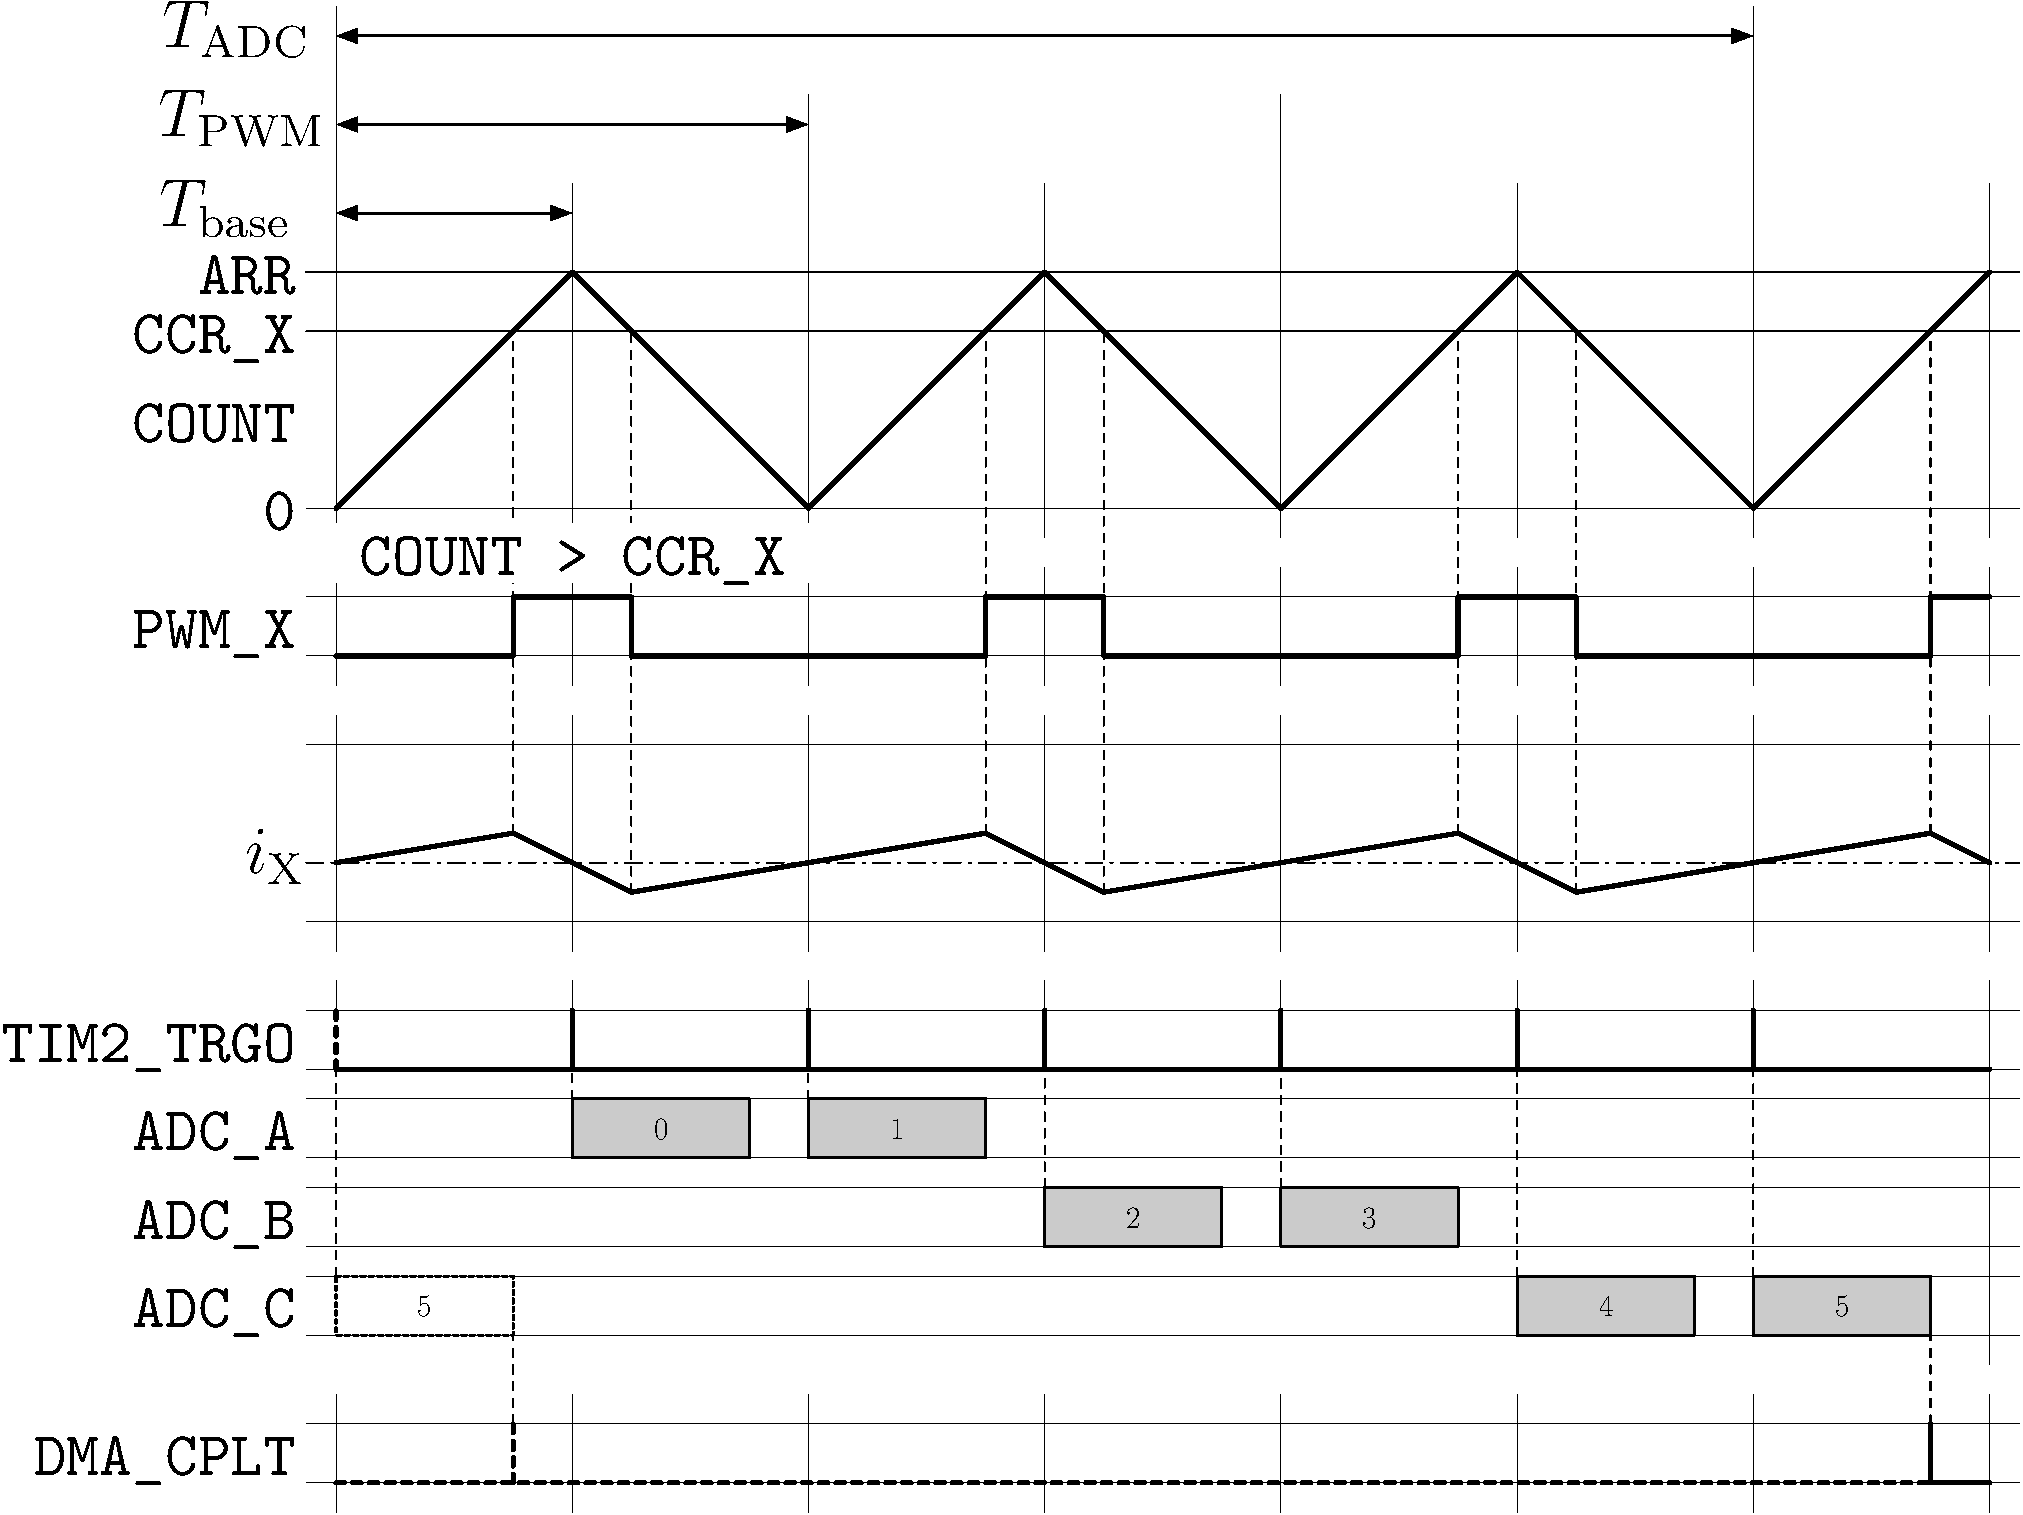
\includegraphics[scale=0.4]{n17-servo-pwm-adc.pdf}
%\caption[PWM and ADC Sync]{Temporal synchronization of PWM output and ADC sampling.}
%\label{fig:pwm-adc}
%\end{center}
%\end{figure}

\subsubsection{ADC Triggering}

As the ADC sampling takes a finite time, it will not quite sample on-center. \texttt{TIM15} is setup to offset by $T_{\textrm{base}} - T_{\textrm{ssaa}}/2 = \unit{6.47}{\micro\second}$ or 1100 CPU cycles.

\begin{figure}[htbp]
\begin{center}
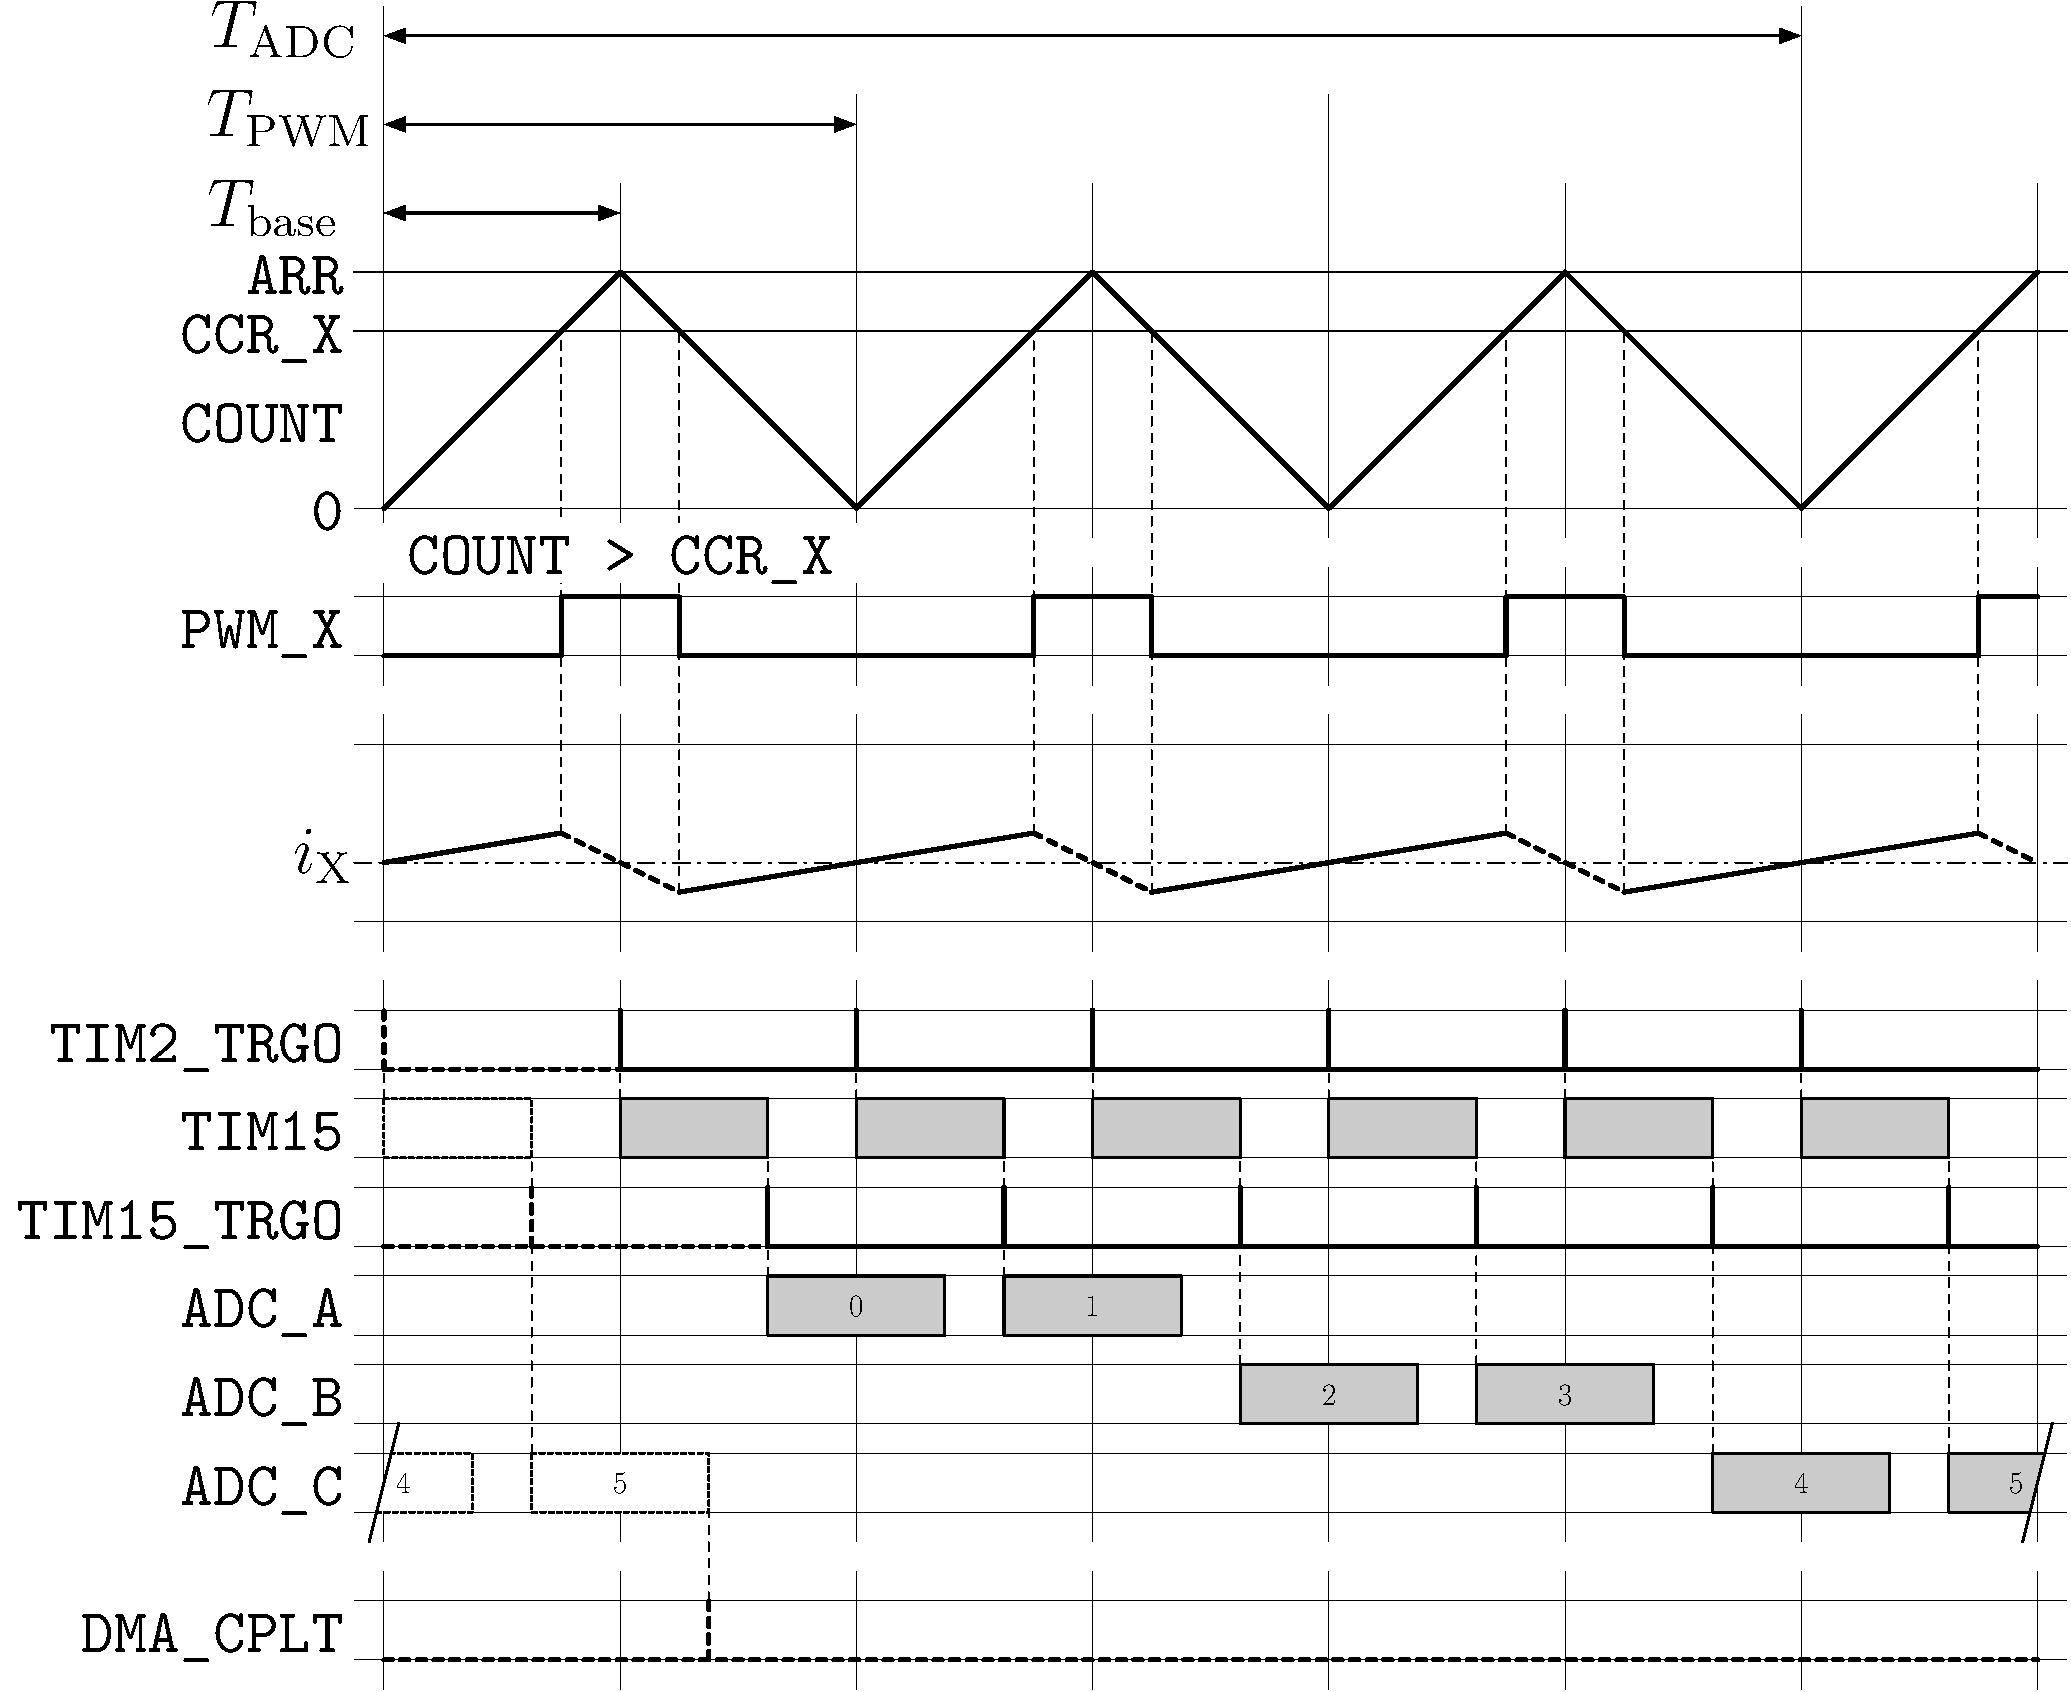
\includegraphics[scale=0.4]{n17-servo-pwm-adc-offset.pdf}
\caption[PWM and ADC Sync with Offset]{Temporal synchronization of PWM output and ADC sampling with centering offset. Adding a triggered timer as a delay allows offsetting the ADC sampling to occur centered on PWM phases.}
\label{fig:pwm-adc-offset}
\end{center}
\end{figure}

\subsection{Sense Resistor Choice}

The \em DRV8323 \em has a programmable gain between 5 and 40, with 20 being the default. 1206-size resistors can dissipate \unit{1}{\watt}\footnote{\unit{2-3}{\watt} according to datasheets for different resistors, so this is with adequate margin}. For \unit{8}{\ampere}, $P = \unit{0.96}{\watt}$ with $R=\unit{15}{\milli\ohm}$. The sense amplifiers can go up to \unit{0.25}{\volt} short of the supply rails, for a \unit{3.3V}{\volt} that leaves \unit{\pm 1.4}{\volt}. The sense voltage $U_S \ @ \  \unit{8}{A}=\unit{120}{\milli\volt}$, thus a gain factor of 5 or 10 would cover the expected current range nicely.

The sense resistor could be made be smaller to reduce power dissipation.

%// 	// default amp gain factor is G = 20 (5/10/20/40) are available
%// 	// current sense shunts are Rs = 15mOhm
%// 	// sense amp output is centered on VREF/2, max. 0.25V away from rail
%// 	// thus +- 1.4V usable range
%// 	// for 12V operation, 10A would give 150mV, factor of 10 gives full range for 8A
%// 	// return Rs * G


\section{PWM}

The PWM output has to be synchronized with sampling the current sense values. This is done through builtin hardware trigger mechanisms between the different peripherals on the MCU which allow precise timing without CPU involvement.

ADC sampling should happen in the middle of the PWM high/low periods, and to achieve this PWM is run in up/down counting mode, and the ADC readout is triggered at the end of each period.

The PWM base period $T_{\textrm{base}} = \unit{10}{\micro\second}$ ($f_{\textrm{base}} = \unit{100}{\kilo\hertz}$) results in an effective output period of $T_{\textrm{gate}} = \unit{20}{\micro\second}$ ($f_{\textrm{gate}} = \unit{50}{\kilo\hertz}$), and ADC sampling of each channel every $T_{\textrm{sense}} = \unit{60}{\micro\second}$ ($f_{\textrm{sense}} = \unit{16.7}{\kilo\hertz}$).

\texttt{TIM2} is setup for driving the gate driver and brake resistor PWM.

\section {ADC}

\subsubsection{ADC Sampling}

\texttt{ADC2} is setup to sample with 12.5 cycles sample time, with 16x oversampling. $f_{\textrm{ADC}} = \unit{170/3}{\mega\hertz}$, and a single channel takes $12.5+12.5$ cycles per sample\footnote{sampling plus conversion}, with $T_{\textrm{sample}} = \unit{0.44}{\micro\second}$. That ends up being $T_{\textrm{ssaa}} = \unit{7.06}{\micro\second}$ with 16x oversampling.

Positive currents can only be measured in low periods, when the lower switch is closed, but negative currents can be measured in both high and low periods, as the body diode will always conduct.

\subsubsection{Sampling High-Impedance Sources}

High-impedance voltage dividers will be affected by ADC input impedance. Longest possible sampling times and additional buffer capacitors at the input are advised.


\section{The RL-Circuit}

\begin{figure}[htbp]
\begin{center}
\begin{circuitikz} \draw
(0,0) to[european voltage source, v=U] (0,4) -- (4,4)
  to[L,l=L,i=i] (4,2)
  to[R,l=R] (4,0) -- (0,0)
;
\end{circuitikz}
\caption[RL Circuit]{RL Circuit Diagram}
\label{fig:RL}
\end{center}
\end{figure}


The governing equation of an RL Series Circuit is 
\begin{align}
\frac{\ud}{\ud t} i &= \frac{U - R i}{L} \\
\frac{\ud^2}{\ud t^2} i &= -\frac{R}{L} \frac{\ud}{\ud t} i
\end{align}
%which can be combined to form
%\begin{align}
%-\frac{L}{R} \frac{\ud^2}{\ud t^2} i &= \frac{U - R i}{L}
%\end{align}
%and simplified to
%\begin{align}
%-\frac{L^2}{R^2} \frac{\ud^2}{\ud t^2} i &= \frac{U}{R} - i\\
%L^2 \frac{\ud^2}{\ud t^2} i &= iR^2 - UR
%\end{align}

\subsubsection{Time Domain}

\begin{align}
i R&= U \left( 1 - e^{-t\frac{R}{L}} \right)
\end{align}


\begin{align}
i &= \frac{U}{R} \left( 1 - e^{-t\frac{R}{L}} \right) \\
\frac{\ud}{\ud t} \imath &= \frac{U}{L} e^{-t\frac{R}{L}} \\
\frac{\ud^2}{\ud t^2} \imath &= -\frac{UR}{L^2} e^{-t\frac{R}{L}}
\end{align}

Logarithmic linear regression of first/second derivative?
\begin{align}
\log \left(\frac{L}{U} \frac{\ud}{\ud t} \imath \right) &= -t\frac{R}{L} \\
\log \left( L \right) - \log \left(U \right) + \log \left(\frac{\ud}{\ud t} \imath \right) &= -t\frac{R}{L} \\
\frac{\ud^2}{\ud t^2} \imath &= -\frac{UR}{L^2} e^{-t\frac{R}{L}}
\end{align}



\subsubsection{Combining for L}

Rearranging both equations to be able to drop $R$
\begin{align}
\frac{R}{L} &= \frac{\frac{U}{L} - \dot{\imath}}{\imath} \\
\frac{R}{L} &= - \frac{ \ddot{\imath}}{ \dot{\imath}}
\end{align}
and combining
\begin{align}
\frac{\frac{U}{L} -  \dot{\imath}}{\imath} &= - \frac{\ddot{\imath}}{ \dot{\imath}} \\
\frac{U}{L} -  \dot{\imath} &= - \frac{\ddot{\imath}}{\dot{\imath}} \imath \\
\frac{U}{L}  \dot{\imath} - \dot{\imath}^2 &= - \ddot{\imath} \imath \\
\frac{U}{L}  \dot{\imath} &= \dot{\imath}^2 - \ddot{\imath} \imath \\
L &= U \frac{ \dot{\imath}}{ \dot{\imath}^2 - \ddot{\imath} \imath}
\end{align}

\subsubsection{Combining for R}
\begin{align}
- R \frac{\dot{\imath}}{\ddot{\imath}} &= U \frac{ \dot{\imath}}{ \dot{\imath}^2 - \ddot{\imath} \imath} \\
- R &= U \frac{ \ddot{\imath}}{ \dot{\imath}^2 - \ddot{\imath} \imath}
\end{align}

\subsubsection{Time Constant}

The above formulas for $R$ and $L$ show that the only difference is the appearance of the first vs. second differential of the current in the nominator. As the current curve is an exponential function, both differentials have the same shape, but differ in magnitude by $\tau=L/R$, and thus 
\begin{align}
\tau &= - \frac{\dot{\imath}}{\ddot{\imath}}
\end{align}

\subsection{R Estimation}

The resistance of the circuit can be easily estimated by applying some low PWM duty cycle long enough to reach steady state, and measuring the current.
\begin{align}
R &= D\frac{U}{\imath}
\end{align}

\subsection{L Estimation with a Known R}

Reformulating
\begin{align}
\frac{\ud}{\ud t} i &= \frac{U - R i}{L}
\end{align}
into
\begin{align}
L &= \frac{U - R i}{\frac{\ud}{\ud t} i}
\end{align}
allows inductance estimation with a relatively simple formula.

\subsection{Impedance Estimation}

Exciting a motor coil with a sinusoidal voltage, and measuring the resulting current phase difference and amplitude, the impedance and thus inductance can be calculated. Assuming a pure sinusoidal signal without harmonics,
\begin{gather}
\begin{aligned}
|Z| &= \frac{U_{\textrm{RMS}}}{i_{\textrm{RMS}}} \\
Z &= R + j X \\
Z &= |Z| \left(\cos \theta + j \sin \theta \right)
\end{aligned}
\end{gather}

\subsubsection{Inductance from Impedance}

\begin{gather}
\begin{aligned}
X &= \sqrt{|Z|^2 - R^2} \\
X_L &= \omega L
\end{aligned}
\end{gather}

It looks like this method yields more accurate results than anything looking at $\frac{\ud}{\ud t} i$. This is not surprising: noise and offsets can be removed more effectively as $L$ is computed from averaged current readings, vs.\ being computed from each individual current reading and then averaged.

This method still seems to over-estimate inductance, but seems to get significantly closer. Interestingly, for a 2-phase motor, the estimated impedance running through both phases gets closer to the specified values than both individual phase measurements.

\subsubsection{Phase Estimation}

The phase angle $\theta$ between $U=U_{\textrm{peak}}\sin \omega$ and $i=i_{\textrm{peak}}\sin \left(\omega+\theta\right)$ can be found as the DC component of the composite signal $U(\omega) \times i(\omega)$:
\begin{gather}
\begin{aligned}
U(\omega) \times i(\omega) &= \frac{\cos \theta - \cos\left(2\omega+\theta\right)}{2} \\
\overline{U \times i} &= \frac{1}{2\pi}\int_0^{2\pi} U \times i \ud \omega = U_{\textrm{peak}} i_{\textrm{peak}}\frac{\cos \theta}{2} \\
\cos \theta &= 2 \frac{\overline{U \times i}}{U_{\textrm{peak}} i_{\textrm{peak}}} =\frac{\overline{U \times i}}{U_{\textrm{RMS}} i_{\textrm{RMS}}}
\end{aligned}
\end{gather}

\subsubsection{Resistance from Impedance and Phase}

\begin{gather}
\begin{aligned}
R &= |Z| \cos \theta = \frac{\overline{U i}}{i_{\textrm{RMS}}^2}
\end{aligned}
\end{gather}

As resistance depends on $R \approx \cos \theta$, it is very sensitive to phase shifts, and thus not very reliable for estimation


\subsection{Simultaneous LR Estimation}

Sampling a  applied voltage $U$ step function at fixed intervals $T$, for samples $i_0, i_1, \ldots, i_n$ with t $t>0,n=t/T$, we can compute the differentiations in different ways.

\subsubsection{N3 Sampling}

Assuming linearity around $n=1$:
\begin{align}
{\imath} &= \frac{1}{3} (\imath_0 + \imath_1 + \imath_2) \\
\dot{\imath} &= \frac{1}{2T} (\imath_2 - \imath_0) \\
\ddot{\imath} &= \frac{1}{T^2} (\imath_2 - 2\imath_1 + \imath_0)
\end{align}
and
\begin{align}
L &= U \frac{\dot{\imath}}{\dot{\imath}^2 - \ddot{\imath} \imath}
\end{align}



\section[2Ph Mot w/ 3Ph Driver]{2-Phase Motor With 3-Phase Driver}

In theory, all motor parameters can be estimated by sequentially turning one half bridge low, while the others are switched high, allowing current to simultaneously flow in in two places, but only out in one. However, the parameter estimation is difficult with noisy values.

\subsection{Full Dynamic Circuit}

\begin{figure}[htbp]
\begin{center}
\begin{circuitikz} 
\draw (0,8) 
  to[R,] ++(0,-2)
  to[normal open switch,] ++(0,-1)
  to[R,] ++(0,-2)
  to[R,] ++(0,-2)
  to[normal open switch,l=$A$] ++(0,-1)
;
\draw (4,8) node[vcc]{U}
  to[R,] ++(0,-2)
  to[normal open switch,] ++(0,-1)
  to[R,] ++(0,-2)
  to[R,] ++(0,-2)
  to[normal open switch,l=$B$] ++(0,-1)
  node[rground]{}
;
\draw (8,8) 
  to[R,l=$R_T$] ++(0,-2)
  to[normal open switch,] ++(0,-1)
  to[R,l=$R_T$] ++(0,-2)
  to[R,l=$R_S$] ++(0,-2)
  to[normal open switch,l=$C$] ++(0,-1)
;
\draw (0,0)
  to[short,-*] ++(4,0)
  to[short] ++(4,0)
;
\draw (0,5)
  to[R,l=$R_P$,*-] ++(2,0)
  to[L,l=$L_P$,] ++(2,0)
  to[R,*-] ++(2,0)
  to[L,-*] ++(2,0)
;
\draw (0,8)
  to[short,-*] ++(4,0)
  to[short] ++(4,0)
;

\end{circuitikz}
\caption[ABBC Driver]{3-Phase Driver with 2-Phase Motor with phase resistance $R_P$ and switching resistance $R_T$ and shunt resistance $R_S$.}
\label{fig:ABBC}
\end{center}
\end{figure}




\begin{figure}[htbp]
\begin{center}
\begin{circuitikz} 
\draw (0,8) 
  to[R,] ++(0,-2)
  to[normal open switch,] ++(0,-1)
  to[R] ++(0,-2)
  to[R,f=$i_A$] ++(0,-2)
  to[short,l=$A$] ++(0,-1)
;
\draw (4,8) node[vcc]{U}
  to[R,f=$i_b$] ++(0,-2)
  to[short,] ++(0,-1)
  to[R,] ++(0,-2)
  to[R,] ++(0,-2)
  to[normal open switch,l=$B$] ++(0,-1)
  node[rground]{}
;
\draw (8,8) 
  to[R,l=$R_T$,f=$i_c$] ++(0,-2)
  to[short,] ++(0,-1)
  to[R,l=$R_T$,] ++(0,-2)
  to[R,l=$R_S$,] ++(0,-2)
  to[normal open switch,l=$C$] ++(0,-1)
;
\draw (0,0)
  to[short,-*] ++(4,0)
  to[short] ++(4,0)
;
\draw (0,5) node[circ,label={[shift={(-0.4,0.0)}]:{$U_a$}}]{}
  to[R,l_=$R_P$,*-] ++(2,0)
  to[L,l_=$L_P$,] ++(2,0) node[circ,label={[shift={(-0.3,0.0)}]:{$U_b$}}]{}
  to[R,-] ++(2,0)
  to[L,-*] ++(2,0) node[circ,label={[shift={(-0.3,0.0)}]:{$U_c$}}]{}
;
\draw (0,8)
  to[short,-*] ++(4,0)
  to[short] ++(4,0)
;

\end{circuitikz}
\caption[ABBC Driver]{Half-Bridge $A$ switched on low, with $B,C$ switched on high creating asymmetric currents across both phases.
}
\label{fig:ABBC-A}
\end{center}
\end{figure}

For the 2-Phase circuit switched as in \cref{fig:ABBC-A} the governing equations with unknowns $i_b,i_c,U_b$ are
\begin{align}
U_b &= L_P \udt i_A + i_A (R_T + R_S + R_P) \\
U-U_b &= i_b R_T \\
U-U_b &= L_P \udt i_c + i_c (R_T + R_P) \\
i_A &= i_b + i_c
\end{align}
and rearranging 
\begin{align}
\udt i_A  &= \frac{U - i_b R_T - i_A (R_T + R_S + R_P)}{L_P} \\
\udt (i_A - i_b)  &= \frac{i_b R_T - (i_A - i_b) (R_T + R_P)}{L_P}
\end{align}
and Laplace transforming
\begin{align}
s I_A(s)  &= \frac{U - I_b(s) R_T - I_A(s) (R_T + R_S + R_P)}{L_P} \\
s \left( I_A(s) - I_b(s) \right) &= \frac{I_b(s) R_T - \left(I_A(s) - I_b(s)\right) (R_T + R_P)}{L_P}
\end{align}
and rearranging
\begin{align}
L_P s I_A(s)  &= U - I_b(s) R_T - I_A(s) (R_T + R_S + R_P) \\
L_P s \left( I_A(s) - I_b(s) \right) &= 2 I_b(s) R_T + I_b(s) R_p - I_A(s) (R_T + R_P)
\end{align}
and again
\begin{align}
R_T I_b(s) &= U - (L_P s + R_T + R_S + R_P) I_A(s)  \\
\left(L_P s + 2 R_T + R_P\right) I_b(s) &= (L_P s + R_T + R_P) I_A(s) 
\end{align}
and combining
\begin{align}
\frac{(L_P s + R_T + R_P)}{L_P s + 2 R_T + R_P} I_A(s)&= \frac{U - (L_P s + R_T + R_S + R_P) I_A(s)}{R_T}
\end{align}
and rearranging
\begin{align}
\left( \frac{(L_P s + R_T + R_P)}{L_P s + 2 R_T + R_P} + \frac{L_P s + R_T + R_S + R_P}{R_T} \right) I_A(s) &= \frac{U}{R_T}
\end{align}
and rearranging
\begin{align}
\left( R_T (L_P s + R_T + R_P) \right. \\
+ &\left (L_P s + R_T + R_S + R_P) (L_P s + 2 R_T + R_P) \right) I_A(s) \\
 = &(L_P s + 2 R_T + R_P) U
\end{align}
expanding
\begin{gather}
\begin{aligned}
\left( R_T L_P s + R_T^2 + R_P R_T \right. \\
+ & L_P^2 s^2 + R_T L_P s + R_S L_P s + R_P L_P s \\
+ & R_T L_P s + 2R_T^2 + R_P R_T \\
+ & R_S L_P s + 2 R_S R_T + R_P R_S\\
+ &\left. R_P L_P s + 2 R_P R_T + R_P^2 \right) I_A(s) \\
 = (L_P s + 2 R_T + R_P) U
\end{aligned}
\end{gather}
simplifying
\begin{gather}
\begin{aligned}
\left( L_P^2 s^2 + 2 R_S L_P s + 2 R_P L_P s + 3 R_T L_P s \right. \\
+ \left. 2 R_S R_T + R_P R_S + R_P^2 + 3 R_T^2 + 4 R_P R_T\right) I_A(s) \\
 = & (L_P s + 2 R_T + R_P) U
\end{aligned}
\end{gather}

\subsection{Resistive Static Circuit}

\begin{figure}[htbp]
\begin{center}
\begin{circuitikz} 
\draw (0,8) 
  to[R,] ++(0,-2)
  to[normal open switch,] ++(0,-1)
  to[R,] ++(0,-2)
  to[R,] ++(0,-2)
  to[normal open switch,l=$A$] ++(0,-1)
;
\draw (4,8) node[vcc]{U}
  to[R,] ++(0,-2)
  to[normal open switch,] ++(0,-1)
  to[R,] ++(0,-2)
  to[R,] ++(0,-2)
  to[normal open switch,l=$B$] ++(0,-1)
  node[rground]{}
;
\draw (8,8) 
  to[R,l=$R_T$] ++(0,-2)
  to[normal open switch,] ++(0,-1)
  to[R,l=$R_T$] ++(0,-2)
  to[R,l=$R_S$] ++(0,-2)
  to[normal open switch,l=$C$] ++(0,-1)
;
\draw (0,0)
  to[short,-*] ++(4,0)
  to[short] ++(4,0)
;
\draw (0,5)
  to[R,l=$R_P$,*-] ++(4,0)
  to[R,*-*] ++(4,0)
;
\draw (0,8)
  to[short,-*] ++(4,0)
  to[short] ++(4,0)
;

\end{circuitikz}
\caption[ABBC Driver Static]{3-Phase Driver with 2-Phase Motor static resistive circuit.}
\label{fig:ABBC-R}
\end{center}
\end{figure}

\begin{figure}[htbp]
\begin{center}
\subfloat[A switched low.]{
\begin{circuitikz} 
\draw (0,8) 
  to[R,] ++(0,-2)
  to[normal open switch,] ++(0,-1)
  to[R] ++(0,-2)
  to[R,f=$i_A$] ++(0,-2)
  to[short,l=$A$] ++(0,-1)
;
\draw (2,8) node[vcc]{U}
  to[R,f=$i_b$] ++(0,-2)
  to[short,] ++(0,-1)
  to[R,] ++(0,-2)
  to[R,] ++(0,-2)
  to[normal open switch,l=$B$] ++(0,-1)
  node[rground]{}
;
\draw (4,8) 
  to[R,l=$R_T$,f=$i_c$] ++(0,-2)
  to[short,] ++(0,-1)
  to[R,l=$R_T$,] ++(0,-2)
  to[R,l=$R_S$,] ++(0,-2)
  to[normal open switch,l=$C$] ++(0,-1)
;
\draw (0,0)
  to[short,-*] ++(2,0)
  to[short] ++(2,0)
;
\draw (0,5)
  to[R,l_=$R_P$,*-*] ++(2,0)
  to[R,-] ++(2,0) 
;
\draw (0,8)
  to[short,-*] ++(2,0)
  to[short] ++(2,0)
;

\end{circuitikz}
}%
~
\subfloat[B switched low.]{
\begin{circuitikz} 
\draw (0,8) 
  to[R,f=$i_a$] ++(0,-2)
  to[short,] ++(0,-1)
  to[R] ++(0,-2)
  to[R,] ++(0,-2)
  to[normal open switch,l=$A$] ++(0,-1)
;
\draw (2,8) node[vcc]{U}
  to[R,] ++(0,-2)
  to[normal open switch,] ++(0,-1)
  to[R,] ++(0,-2)
  to[R,f=$i_B$] ++(0,-2)
  to[short,l=$B$] ++(0,-1)
  node[rground]{}
;
\draw (4,8) 
  to[R,l=$R_T$,f=$i_c$] ++(0,-2)
  to[short,] ++(0,-1)
  to[R,l=$R_T$,] ++(0,-2)
  to[R,l=$R_S$,] ++(0,-2)
  to[normal open switch,l=$C$] ++(0,-1)
;
\draw (0,0)
  to[short,-*] ++(2,0)
  to[short] ++(2,0)
;
\draw (0,5)
  to[R,l_=$R_P$,*-*] ++(2,0)
  to[R,-] ++(2,0) 
;
\draw (0,8)
  to[short,-*] ++(2,0)
  to[short] ++(2,0)
;

\end{circuitikz}
}
\caption[ABBC-RAB]{Resistive Half-Bridge switched low on $A,B$ phases, respectively.
}
\label{fig:ABBC-RAB}
\end{center}
\end{figure}

For the 2-Phase circuit switched as in \cref{fig:ABBC-RAB} the measureable resistances are
\begin{gather}
\begin{aligned}
R_A &= R_S + R_T + R_P + \frac{R_T (R_T + R_P)}{2 R_T + R_P} \\
R_B &= R_S + R_T + \frac{R_T + R_P}{2}
\end{aligned}
\end{gather}
which allows us to solve for $R_T, R_P$ with $R_S$ being known:
\begin{gather}
\begin{aligned}
(2 R_T + R_P) (R_A - R_S - R_T - R_P) &= R_T (R_T + R_P) \\
R_P &= 2 R_B - 2 R_S - 3 R_T
\end{aligned}
\end{gather}
and combining the two equations to solve for $R_T$
\begin{gather}
\begin{aligned}
(2 R_B - 2 R_S - R_T) (R_A + R_S + 2 R_T - 2 R_B) &= R_T (2 R_B - 2 R_S - 2 R_T) \\
2 R_A R_B + 2 R_B R_S + 4 R_B R_T - 4 R_B^2 \\
 - 2 R_A R_S - 2 R_S^2 - 4 R_S R_T + 4 R_B R_S\\
 - R_A R_T - R_S R_T - 2 R_T^2 + 2R_B R_T &= 2 R_B R_T - 2 R_S R_T - 2 R_T^2 \\
2 R_A R_B - 4 R_B^2 - 2 R_A R_S - 2 R_S^2 + 6 R_B R_S &= R_A R_T + 3 R_S R_T - 4 R_B R_T\\
2 \frac{ R_A R_B - 2 R_B^2 - R_A R_S - R_S^2 + 3 R_B R_S}{R_A + 3 R_S- 4 R_B} &= R_T\\
2 \frac{ 2 R_B^2 - R_A R_B  + R_A R_S - 3 R_B R_S + R_S^2}{4 R_B - R_A - 3 R_S} &= R_T\\
\end{aligned}
\end{gather}
and for $R_P$
\begin{gather}
\begin{aligned}
2 \frac{ 2 R_B^2 - R_A R_B  + R_A R_S - 3 R_B R_S + R_S^2}{4 R_B - R_A - 3 R_S} &= \frac{R_P - 2 R_B + 2 R_S}{3} \\
\frac{ 12 R_B^2 - 6 R_A R_B  + 6 R_A R_S - 18 R_B R_S + 6 R_S^2}{4 R_B - R_A - 3 R_S} + 2 R_B - 2 R_S &= R_P \\
\frac{ 20 R_B^2 - 8 R_A R_B  + 8 R_A R_S - 32 R_B R_S + 12 R_S^2}{4 R_B - R_A - 3 R_S} &= R_P \\
4 \frac{ 5 R_B^2 - 2 R_A R_B  + 2 R_A R_S - 8 R_B R_S + 3 R_S^2}{4 R_B - R_A - 3 R_S} &= R_P
\end{aligned}
\end{gather}

\subsection{Single Current Path}

System identification  with only one active high and low switch at a time, and the third half-bridge being disabled, results in simpler equations than having two active high switches:
\begin{gather}
\begin{aligned}
R_{AB} = R_{BC} &= R_P + 2 R_T + R_S \\
R_{AC} &= 2 R_P + 2 R_T + R_S \\
\end{aligned}
\end{gather}

\subsection{2-Phase Driving}

Because the 2 phases share a common point, the maximum available voltage is limited to less than the line voltage. It is assumed that the phases are driven sinusoidally with a $\frac{\pi}{2}$ phase shift.

With a naive approach of keeping the center point at half the nominal voltage, only half the nominal voltage is available for each phase. Moving the midpoint, too, allows us to increase phase voltage to $U_P = \sqrt{2} U$, with the following waveforms:
\begin{gather}
\begin{aligned}
U_{A} &= \frac{\cos x}{\sqrt{2}} \\
U_{C} &= \frac{\sin x}{\sqrt{2}} \\
U_{B} &= \frac{\cos x + \sin x}{4} = \frac{\cos \left(x - \frac{\pi}{4}\right)}{2 \sqrt{2}}
\end{aligned}
\end{gather}
and PWM
\begin{gather}
\begin{aligned}
D_{A} &= U_{B} + U_{A} \\
D_{B} &= U_{B} \\
D_{C} &= U_{B} + U_{C}
\end{aligned}
\end{gather}

The physical limiting condition to observe is that 
\begin{gather}
\begin{aligned}
\forall \left( U_{A}+U_{B} \right) &\leq U_P
\end{aligned}
\end{gather}

\section{Position Estimation}

\subsection{Discrete Kalman Filter}

\subsubsection{Difference Equation}

Variable names after \cite{kalman-tut} with slight adjustments. The discrete stochastic time-variant system is described by
\begin{gather}
\begin{aligned}
\vx_k &= \mA_{k} \vx_{k-1} +  \mB_{k} \vu_{k-1} + \vw_{k-1} \\
\vz_k &= \mH_k \vx_k + \vv_k
\end{aligned}
\end{gather}
where \vx\ is the state vector, \vu\ is the input vector, \vz\ is the observation vector, and \vw\ and \vv\ are the process and measurement noise vector vectors, respectively, for a given time step $k$.

$\mH$ maps the state to the observable variables, and features prominently in the Kalman Filter equations.

The noise vectors are defined by the corresponding covariance matrices $\mQ_k$ and $\mR_k$. The state covariance matrix is $\mP_k$.

\subsubsection{Canonical Kalman Filter Update}

The first part of the update is prediction
\begin{gather}
\begin{aligned}
\vx^-_k &= \mA \vx^+_{k-1} +  \mB \vu_{k-1} \\
\mP^-_k &= \mA\mP^+_{k-1}\mA^T + \mQ
\end{aligned}
\end{gather}
which results in the \em a-priori \em (as in before measurement) estimates of $\vx^-, \mP^-$. The second part is the correction through measurement
\begin{gather}
\begin{aligned}
\mK &= \mP^-_k\mH^T\left( \mH \mP^-_k \mH^T + \mR \right)^{-1}\\
\vx^+_k &= \vx^-_k + \mK \left(\vz_k - \mH\vx^-_k \right)\\
\mP^+_k &= \left( \mI - \mK \mH \right) \mP^-_k
\end{aligned}
\end{gather}
resulting in the \em Kalman Gain \em $\mK$, and \em a-posteriori \em (post measurement) estimates of the state vector $\vx^+, \mP^+$.

In this form, the computation of $\mK$ requires a matrix inversion. If the process and measurement noise covariance matrices are constant, the inversion can be avoided by pre-computing the state covariance matrix $\mP$ with the Ricatti Equation. In our case, however, both $\mQ$ and $\mR$ are time-dependent.

\subsubsection{DC Motor State Equation}

The electrical and mechanical DC motor model with the parameters of  electrical motor constant $k_e$, rotor inertia $J$, resistance $k_d$, and disturbance torque $\Gamma_d$:

\begin{gather}
\begin{aligned}
L\frac{\ud }{\ud t} \imath&= U - R \imath - k_e \omega \\
J \frac{\ud }{\ud t} \omega &= k_e \imath - k_d \omega - \Gamma_d \\
\frac{\ud}{\ud t} x &= \omega
\end{aligned}
\end{gather}

\subsubsection{Simplest Approximation Difference Equations}

In the simplest possible form, the motor can be treated as an inertial mass without outside forces, eg.{} it having constant speed.

\begin{gather}
\begin{aligned}
\omega &= \frac{\ud}{\ud t} x
\end{aligned}
\end{gather}

This is a useful approximation if further motor parameters that link the electrical and mechanical models are unknown, but has the big drawback that changes in speed cannot be modeled well. Therefore, this model is only useful to determine motor position and speed from the position encoder during system identification, but not during regular operation.

The mechanical position $x$ of the motor and its speed $\omega$ compromise the state vector. There are no inputs, and the only available measurement is the measured position $x'$:
\begin{gather}
\begin{aligned}
\vx &= \left(
\begin{array}{c}
      x  \\
 \omega \\
%\ddot{x}   
\end{array}
\right) \\
%\vu &= \left(
%\begin{array}{c}
%      \imath
%\end{array}
%\right) \\
\vz &= \left(
\begin{array}{c}
      x'
\end{array}
\right)
\end{aligned}
\end{gather}
The update/correction matrices depend only on the time step size $h$:
\begin{gather}
\begin{aligned}
\mA &= \left(
\begin{array}{cc}
 1 & h \\
 0 & 1 \\
\end{array}
\right) \\
%\mB &= \left(
%\begin{array}{c}
% k_T \frac{h^2}{2} \\
% k_T h   
%\end{array}
%\right) \\
\mH &= \left(
\begin{array}{c c}
 1 & 0
\end{array}
\right).
\end{aligned}
\end{gather}
Without inputs, $\mB\vu = 0$ and can be ignored.

The covariance matrices are the most difficult to determine. We need to take into account the effects of the applied voltage $U$ and/or current $\imath$, and balance the model and measurement covariances to get a stable prediction, but also a fast enough reaction, though such a filter will invariable react more slowly to changes than a more complete model. In addition to $h$, we might also consider the change in input voltage $\frac{\ud}{\ud t} U$ and time since the last observation $\lambda$
\begin{gather}
\begin{aligned}
%\mP &= \left(
%\begin{array}{cc}
% ? & 0 \\
% 0 & ? \\
%\end{array}
%\right) \\
\mQ &= \left(
\begin{array}{cc}
 \left( k_{Q1} h \right)^2 & 0 \\
 0 & \left( k_{Q2} h \right)^2
\end{array}
\right) \\
\mR &= \left(
\begin{array}{c}
 \left( k_{R1} + k_{R2} \lambda + k_{R3} \omega \lambda \right)^2\\
\end{array}
\right)
\end{aligned}
\end{gather}
For $\mR$, we will have a noise figure from the sensor to determine $k_{R1}$. $k_{R2}$ expresses how much we trust the measurement as time goes on without further information, and $k_{R2}$ expresses uncertainty it terms of rotational speed.

If the motor that isn't being driven, what is the expected amount we expect it to move? For a stepper motor, we expect it might clog to the next full step. If it is moving, and we expect it to continue so without further input, it will have moved $\omega \lambda$ plus some unmodeled effect from potential friction. 

The uncertainty in the process might quantified by taking into account potential forces that are not accounted for in the model. Neglecting external forces, we have control over our target speed $\omega$ and the acceleration $\alpha_{\textrm{max}}$.

For a scalar $R$, due to only having a single observed variable, $\mK$ can be calculated straight-forwardly without a matrix inversion.

\begin{table}[htbp]
\caption{Covariance parameters for constant speed motor model.}
\begin{center}
\begin{tabular}{llp{0.5\textwidth}} \toprule
 Parameter & Value & Comment \\
\midrule
$k_{Q1}$ & $0.2\pi$ & \unit{10}{\%} of $\alpha_{\textrm{max}}$ as unmodeled disturbance\\
$k_{Q2}$ & $2\pi$ & larger uncertainty in speed, due it being derived from position\\
$k_{R1}$ & $0.0222$  & ONL $\sigma = \unit{0.068}{\degree}$ + INL $ = \unit{1.2}{\degree}$\\
$k_{R2}$ & $2\pi$ & $\alpha_{\textrm{max}} = \unit{2\pi}{\radian\per\second\squared}$ acc limit \\
$k_{R3}$ & $0$ & assuming measurement is compensated by speed est. \\
\bottomrule
\end{tabular}
\end{center}
\label{tab:cov-params-const-speed}
\end{table}%


\nocite{*}

%\bibliographystyle{ieeetr}
%\bibliography{n17-servo-design}
\printbibliography


\end{document}


